%  article.tex (Version 3.3, released 19 January 2008)
%  Article to demonstrate format for SPIE Proceedings
%  Special instructions are included in this file after the
%  symbol %>>>>
%  Numerous commands are commented out, but included to show how
%  to effect various options, e.g., to print page numbers, etc.
%  This LaTeX source file is composed for LaTeX2e.

%  The following commands have been added in the SPIE class 
%  file (spie.cls) and will not be understood in other classes:
%  \supit{}, \authorinfo{}, \skiplinehalf, \keywords{}
%  The bibliography style file is called spiebib.bst, 
%  which replaces the standard style unstr.bst.  

%\documentclass[]{spie}  %>>> use for US letter paper
\documentclass[a4paper, 11pt, twocolumn]{spie}  %>>> use this instead for A4 paper
%%\documentclass[nocompress]{spie}  %>>> to avoid compression of citations
%% \addtolength{\voffset}{9mm}   %>>> moves text field down
%% \renewcommand{\baselinestretch}{1.65}   %>>> 1.65 for double spacing, 1.25 for 1.5 spacing 
%  The following command loads a graphics package to include images 
%  in the document. It may be necessary to specify a DVI driver option,
%  e.g., [dvips], but that may be inappropriate for some LaTeX 
%  installations. 
\usepackage[]{times}
\setlength{\columnsep}{0.8cm}
\usepackage{titlesec}


\titleformat{\section}[runin]{\normalfont\bfseries}{\thesection.}{1em}{}
\titleformat{\subsection}[runin]{\normalfont\bfseries}{\thesubsection.}{1em}{}

\titlespacing{\section}{0pt}{6pt}{5pt}
\titlespacing{\subsection}{0pt}{3pt}{5pt}

\clubpenalty=10000 % to kara za sierotki
\widowpenalty=10000 % nie pozostawia wdów
\brokenpenalty=10000 % nie dzieli wyrazów pomiędzy stronami
\usepackage[
top    = 5.2cm,
bottom = 3.0cm,
left   = 2.50cm,
right  = 2.50cm]{geometry}



\pagenumbering{arabic}

\usepackage{secdot}
\usepackage[]{graphicx}

%\usepackage[polish]{babel}
\usepackage[utf8x]{inputenc}	% polish letters (for names)
%\usepackage[T1]{fontenc}
\usepackage{mathtools}			% matrix*
\usepackage{booktabs}			% professional tables
\usepackage[]{amsmath}

\newcommand{\bm}[1]{\boldsymbol{#1}}

\title{Implementation aspects of Graph Neural Networks}

%>>>> The author is responsible for formatting the 
%  author list and their institutions.  Use  \skiplinehalf 
%  to separate author list from addresses and between each address.
%  The correspondence between each author and his/her address
%  can be indicated with a superscript in italics, 
%  which is easily obtained with \supit{}.

\author{
Aleksy Barcz\\
{\normalsize Institute of Computer Science, Warsaw University of Technology,\\
ul. Nowowiejska 15/19, 00-665 Warsaw, Poland.\\
abarcz@gmail.com}
}

%>>>> Further information about the authors, other than their 
%  institution and addresses, should be included as a footnote, 
%  which is facilitated by the \authorinfo{} command.

\authorinfo{}
%%>>>> when using amstex, you need to use @@ instead of @
 

%%%%%%%%%%%%%%%%%%%%%%%%%%%%%%%%%%%%%%%%%%%%%%%%%%%%%%%%%%%%% 
%>>>> uncomment following for page numbers
\pagestyle{plain}    
%>>>> uncomment following to start page numbering at 301 
%\setcounter{page}{301} 
 
\begin{document} 
\maketitle 

%%%%%%%%%%%%%%%%%%%%%%%%%%%%%%%%%%%%%%%%%%%%%%%%%%%%%%%%%%%%% 
\begin{abstract}
\emph{This report summarises the results of implementation of a Graph Neural Network~\cite{scarselli2009graph} classifier. As a quite new neural network model, GNN still seems to lack a thorough analysis, which would take into account all aspects of GNN implementation and parameters adjustment. This report describes some aspects of GNN behaviour, related to its parameters and implementation details.}
\end{abstract}

%>>>> Include a list of keywords after the abstract 


%%%%%%%%%%%%%%%%%%%%%%%%%%%%%%%%%%%%%%%%%%%%%%%%%%%%%%%%%%%%%
\section{Introduction.}
The Graph Neural Network model is a connectionist classifier capable of classifying graphs. Most of the other existing neural network-based graph classifiers, such as RAAM~\cite{pollack1990recursive} or  LRAAM~\cite{sperduti1994labelling} and all solutions basing on them are capable of processing certain types of graphs only, in most cases DAGs (directed acyclic graphs) or DPAGs (directed positional acyclic graphs).Several solutions were invented to deal with cyclic graphs, such as introducing a delay in the LRAAM encoding tree~\cite{goulon2005hopfield} or techniques mapping cyclic directed graphs to "recursive equivalent" trees~\cite{bianchini2003backpropagation}. The problem of nonpositional graphs was also addressed by several authors, either by creating domain-specific encodings used to enforce a defined order on graph nodes~\cite{ivanciuc2003canonical} or by introducing various modifications to the classifier~\cite{bianchini2005recursive}. However, most of the solutions dealing with cyclic and nonpositional graphs either complicate the classifier model, enlarge the input dataset or (in case of cycles) may result in information loss. The Graph Neural Network model can directly process most types of graphs, including cyclic, acyclic, directed, undirected, positional and nonpositional, which makes it a flexible solution. There is a conceptual similarity between the GNN model and Graph Machines~\cite{goulon2005learning}, however the GNN model adapt a different learning and backpropagation schema which simplifies processing different types of graphs. This report describes the steps of implementation of a GNN classifier, including some details which were not described in the original article~\cite{scarselli2009graph}. The classifier was implemented in GNU Octave with two ideas in mind: providing a simple interface (similar to that of the Neural Networks toolbox) and maximum flexibility, that is the possibility of processing each kind of data that the theoretical model could deal with. At the end some classification results are presented. Notation from the original article describing GNNs~\cite{scarselli2009graph} was used where applicable.

\section{Input data.}
The input graph data consisted of: node labels ($l_n, |l_n| \geq 1$), edge labels ($l_{(n,u)}, |l_{(n,u)}| \geq 0$) and node outputs ($o_n, |o_n| \geq 1$). Each edge was described by its label and two node indexes: source node and target node. For directed and undirected edges a schema different from the original one was adapted. Usually a directed edge in a graph means that each of its nodes influence the other one equally, therefore directed edges were represented as pairs of directed edges, so the GNN could treat equally both nodes from a single edge.

\section{Computation units.}
The GNN classifier is built using two separate computation units: $f_w$ and $g_w$. The $f_w$ unit is used to build representation of the graphs nodes (the \emph{state} $x_n$), while the $g_w$ unit processes the obtained representation, producing output that should match the expected output $o_n$ for the nth node. The nonpositional form of $f_w$ was selected as the more general one and the one performing better at the evaluation tasks~\cite{scarselli2009graph}. To prove the capability of building a representation sufficiently encoding both node and graph structure information, minimal form of $f_w$ and $g_w$ was chosen as shown in Eq.~\ref{eq:hw} and Eq.~\ref{eq:gw}.

\newgeometry{top=3cm,bottom=3cm,right=2.5cm,left=2.5cm} \noindent
The $f_w$ unit was implemented as a simple sum of the $h_w$ unit output evaluated at each directed edge $(n, u)$, connecting node $u$ to the node $n$. All instances of the $h_w$ unit share their weights and all instances of the $g_w$ unit share their weights. 


\begin{equation}
x_n = \sum_{u \in ne[n]} h_w(l_n, l_{(n, u)}, x_u)
\label{eq:hw}
\end{equation}

\begin{equation}
o_n = g_w(x_n)
\label{eq:gw}
\end{equation}
Both $h_w$ and $g_w$ units were implemented as three layer feedforward neural networks (inputs, hidden layer, output layer). In both units the hidden layers were composed of $tanh$ neurons. In the $h_w$ unit the output layer was composed of $tanh$ neurons to assure that the state $x_n$, which was later passed to the $g_w$ network, consisted of bounded values only. The output layer of the $g_w$ unit could be configured either as a layer with $tanh$ activation function or a layer of linear neurons. The weights of both the $h_w$ and $g_w$ units were initialised according to standard neural network practice, to avoid saturation of any $tanh$ activation function: $net_j = \sum_i w_{ij} y_i \in (-1, 1)$. The initial input weights of the $g_w$ unit were divided by an additional factor, i.e. the maximum node indegree of the processed graphs, to take into consideration the fact, that the input of $g_w$ unit consists of a sum of $h_w$ outputs. All the input data (node and edge labels) was normalised appropriately.

\begin{figure}
\begin{center}
	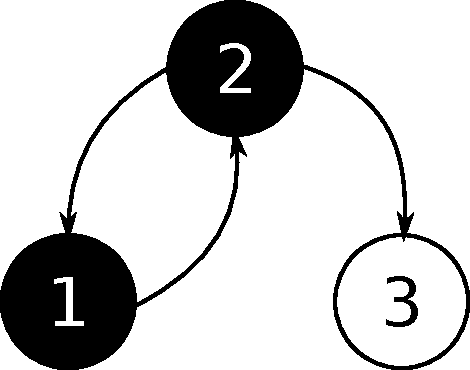
\includegraphics[scale=0.4]{img/graph_classes}
	\caption{Sample graph with nodes belonging to two classes and the corresponding encoding network}
	\label{fig:graph}
\end{center}
\end{figure}

\begin{figure}
\begin{center}
	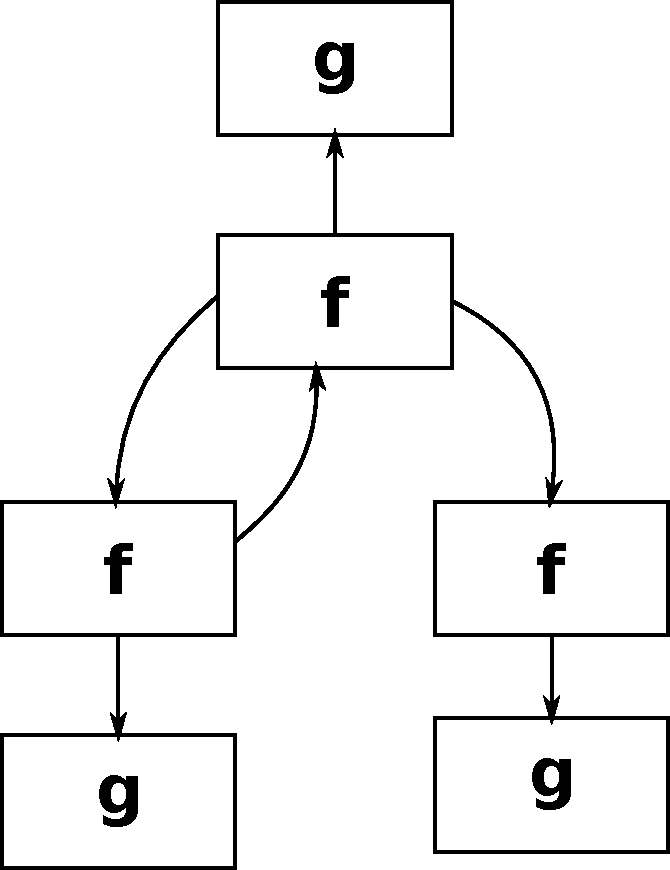
\includegraphics[scale=0.4]{img/encoding_thin}
	\caption{Encoding network for the sample graph}
	\label{fig:enc}
\end{center}
\end{figure}

\section{Learning algorithm.}
The learning algorithm for GNNs was implemented as follows:
\begin{enumerate}
	\item initialize $h_w$ and $g_w$ weights
	\item for predefined number of steps:
	\begin{enumerate}
		\item FORWARD: initialize X randomly and calculate X = F(X) until fixed point is reached
		\item BACKWARD: calculate G(X), backpropagate the error and calculate penalty
		\item update weights using RPROP~\cite{riedmiller1993direct} algorithm
	\end{enumerate}
\end{enumerate}

\subsection{Forward.}
The computation of fixed point $X$ was implemented according to the original source. The encoding network, consisting of identical copies of the $f_w$ unit, connected according to graph topology, was being unfolded in time up to a point, where the state reaches fixed point. The process of reaching fixed point in computation of the state can be viewed as performing time steps, where at each time step we evaluate $f_w$ at each node of the graph and the graph edges are taken into consideration only between time steps~(Fig.~\ref{fig:forward}). Random initialisation of the state $X$ at the beginning of each FORWARD call proved to work well. However number of steps necessary to reach fixed point could vary a lot - from about 5 to 40 steps when $F_w$ was indeed a contraction map to several thousands and probably more (computation was interrupted due to excessive time) when $F_w$ was losing its contraction features. Therefore, for the sake of conducting experiments in predictable time, a maximum number of steps for the unfolding phase was introduced (\emph{maxForwardSteps}) and set to 200 for all the subsequent experiments. This value was chosen according to number of steps made usually by the FORWARD phase during the previous experiments, to allow reaching the fixed point.
\newpage \noindent It was observed that even when the algorithm reached the maximum number of steps and the calculation of $X$ was interrupted and therefore not exact (and also when $F_w$ most probably ceased to be a contraction map), the learning algorithm was still able to perform quite well. In most cases, the RMSE error didn't increase significantly or even continued to drop.


\subsection{Backward.}
The error backpropagation algorithm was implemented according to the original source, in a way similar to the Almeida-Pineda algorithm~\cite{williams1995gradient} designed for BPTT. The error of $g_w$ unit was backpropagated through the unfolded network and also injected at each time step (Fig.~\ref{fig:backward}). In such a way every "layer" of $f_w$ units at a given timestep $t_i$ was provided with two kinds of error - the error coming from the subsequent timesteps of the unfolded network and also the error that would have been backpropagated to the $f_w$ units directly from the $g_w$ units if the unfolding had been stopped after the timestep $t_i$. According to this schema, it should be noted that the initial value of the error accumulator $z_0$~\cite{scarselli2009graph} should be set to the error backpropagated through the $g_w$ layer. As the error backpropagation in the Almeida-Pineda algorithm is recurrent, a maximum number of steps for error accumulation was introduced (\emph{maxBackwardSteps}) and set to 200, as the maximum number of forward steps. However the number of backward steps proved to be smaller than the number of forward steps and rarely reached the maximum value.

\subsection{RPROP algorithm.}
The GNN learning algorithm produces at the end of the BACKWARD phase two kinds of weight updates:$\frac{\partial e}{\partial w}$ and $\frac{\partial p}{\partial w}$. The first is the error calculated by Almeida-Pineda algorithm for $h_w$ and $g_w$. The second is the derivative of penalty imposed on $h_w$~weights to make $F_w$ a contraction map, when $F_w$ ceases to be one. The corresponding $\frac{\partial e}{\partial w}$ and $\frac{\partial p}{\partial w}$ errors are summed up to form the final weight update which would normally be used to update the weights in a standard neural network learning algorithm. However, it occurs that the term $\frac{\partial p}{\partial w}$ can sometimes be several orders of magnitude larger than the $\frac{\partial e}{\partial w}$ term, a disproportion that could render the traditional gradient descent algorithm useless. Therefore the RPROP algorithm must be used, not only to make the gradient descent fast~\cite{scarselli2009graph}, but also to make it robust against the potentially unforseeable behaviour of the  $\frac{\partial e}{\partial w}$ term. Some early experiments with standard gradient descent algorithm confirmed that when $\frac{\partial p}{\partial w}$ was applied directly to weights, the learning algorithm couldn't reach its target, while introducing the RPROP algorithm fixed that issue. The RPROP algorithm was implemented using standard recommended values~\cite{riedmiller1993direct}, with the exception of $\Delta_{max}$ which was set to $1$ to avoid large weight changes.

\begin{figure}
\begin{center}
	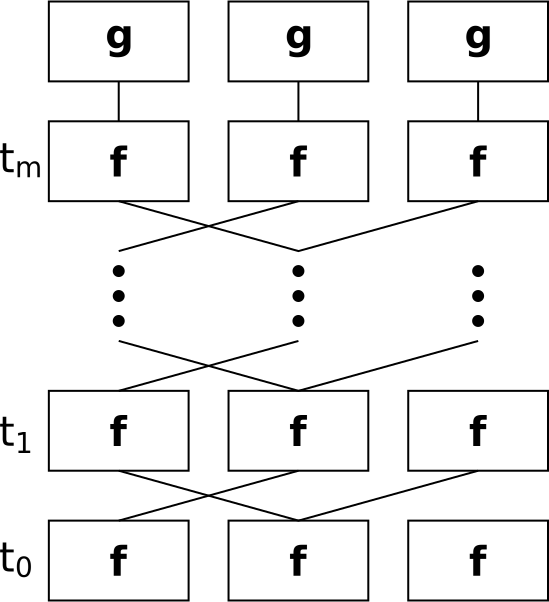
\includegraphics[scale=0.4]{img/forward}
	\caption{Encoding network unfolded}
	\label{fig:forward}
\end{center}
\end{figure}


\begin{figure}
\begin{center}
	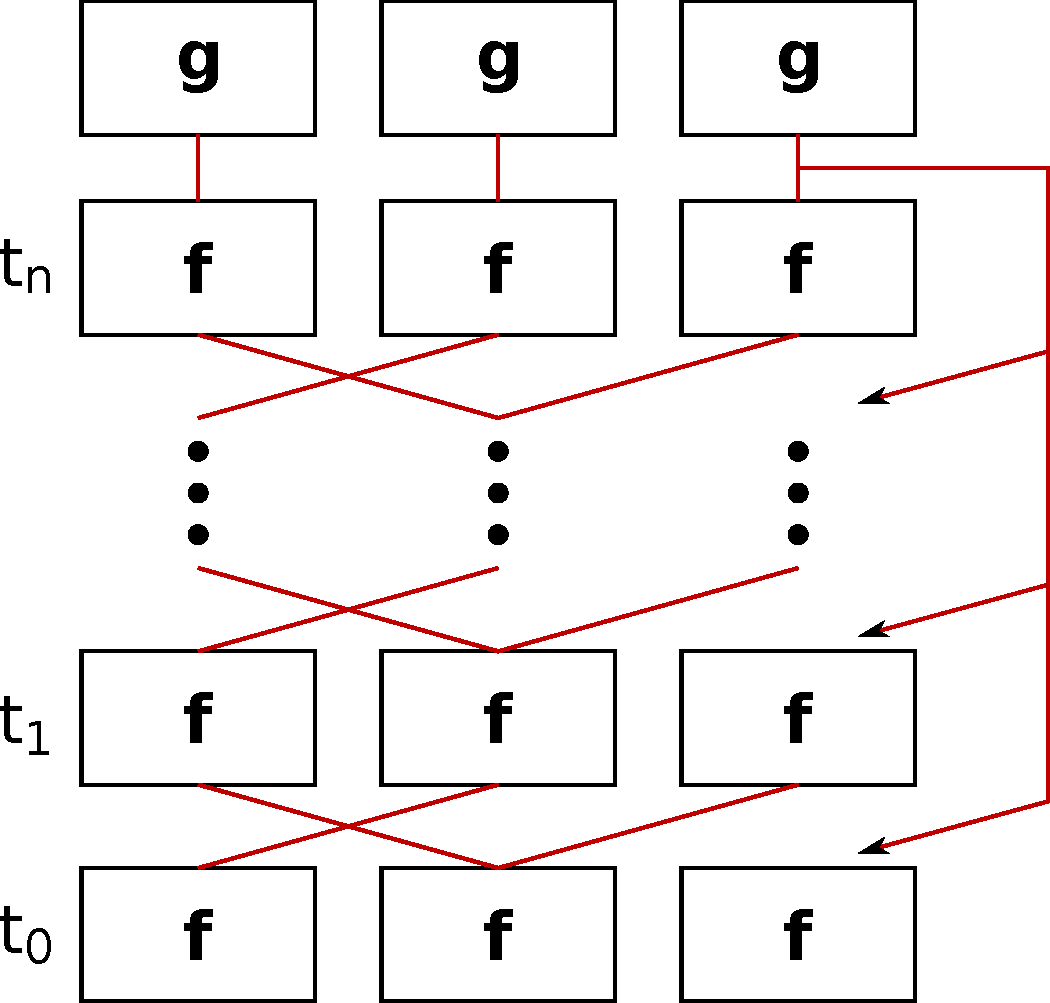
\includegraphics[scale=0.4]{img/backward}
	\caption{Error backpropagation}
	\label{fig:backward}
\end{center}
\end{figure}

\newpage
\section{Influence of contraction constant.}
Weights of the $h_w$ unit are penalized when the impact of a state $x_u$ (used as input for $f_w$) on \emph{j}th element of state $x_n$ becomes too large (impact summed over all nodes $n$ for which exists an edge from $x_u$ to $x_n$). Contraction constant $\mu$ controls how early a penalty will be imposed on $h_w$ weights (in the case when $F_w$ stops being a contraction map) and how large that penalty will be. More precisely, a larger $\mu$ will impose the penalty after a larger impact occurred and the impact will be smaller (Eq.~\ref{eq:contraction}).

\begin{equation}
L\left(I_{n,j} - \mu\right) = \left\{
	\begin{array}{l l}
		I_{n,j} - \mu & \quad \text{if} \quad I_{n,j} > \mu \\
		0 & \quad \text{otherwise}
	\end{array} \right. ,
\label{eq:contraction}
\end{equation}

\begin{equation}
I_{n,j} = \sum_{(n, u) \in E} \sum_{i=1}^{s}|A_{n,u}^{i,j}|.
\end{equation}

Experiments were made using the subgraph matching problem (dataset similar to the one used in the original article~\cite{scarselli2009graph}). Dataset consisted of 20 random graphs, 6 nodes per graph (node labels [0..10]), edges inserted with probability 0.8. A subgraph with 3 nodes was inserted to each graph. The task for the GNN was to decide whether a given node in a graph belongs to the subgraph or not. Three different values of $\mu$ were applied to the same GNN during training (same initial weights): [1.2, 0.9, 0.6]. The experiment was repeated 10 times using two initial weights sets. It appeared that in most cases the best learning results were obtained using $\mu = 0.9$ or $\mu = 1.2$, while using $\mu = 0.6$ usually resulted in a lack of learning (RMSE on training set didn't decrease). This suggests that for a given problem there exists a minimal value of $\mu$, below which the classifier doesn't learn well. The problem seems to be twofold. First, when the value of $\mu$ is too small, the penalty is imposed not only when $F_w$ stops being a contraction map (we can with a certain probability deduce the lack of contraction from the number of FORWARD steps), which disturbs the learning process. Second, a larger value of penalty more easily overcomes the $\frac{\partial e}{\partial w}$ term, which also disturbs the learning process, as the weight updates made by RPROP will have the sign of the penalty term. Fig.~\ref{fig:rmse1}, fig.~\ref{fig:rmse2}, fig.~\ref{fig:rmse3} show RMSE on training set for a single GNN trained with different contraction constants. Figure~\ref{fig:rmse1} shows in details the process of training with $contractionConstant = 1.2$. For $\mu = 1.2$ it was observed that the penalty wasn't used as often as it could - when the number of Forward steps reached its maximum. Also, the influence of $\frac{\partial e}{\partial w}$ was significant and never dropped below 60\%. It could be seen that the decrease of RMSE error was justified - even if the number of Forward steps reached its maximum most of the time, the GNN was still able to accumulate all the error in a finite number of Backward steps. Different behaviour was observed with $\mu = 0.6$. The penalty was imposed even when the number of Forward steps was below maximum. The influence of $\frac{\partial e}{\partial w}$ was constantly below 80\% and was dropping even below 50\%. This resulted in a lack of learning.

\begin{figure}
\begin{center}
	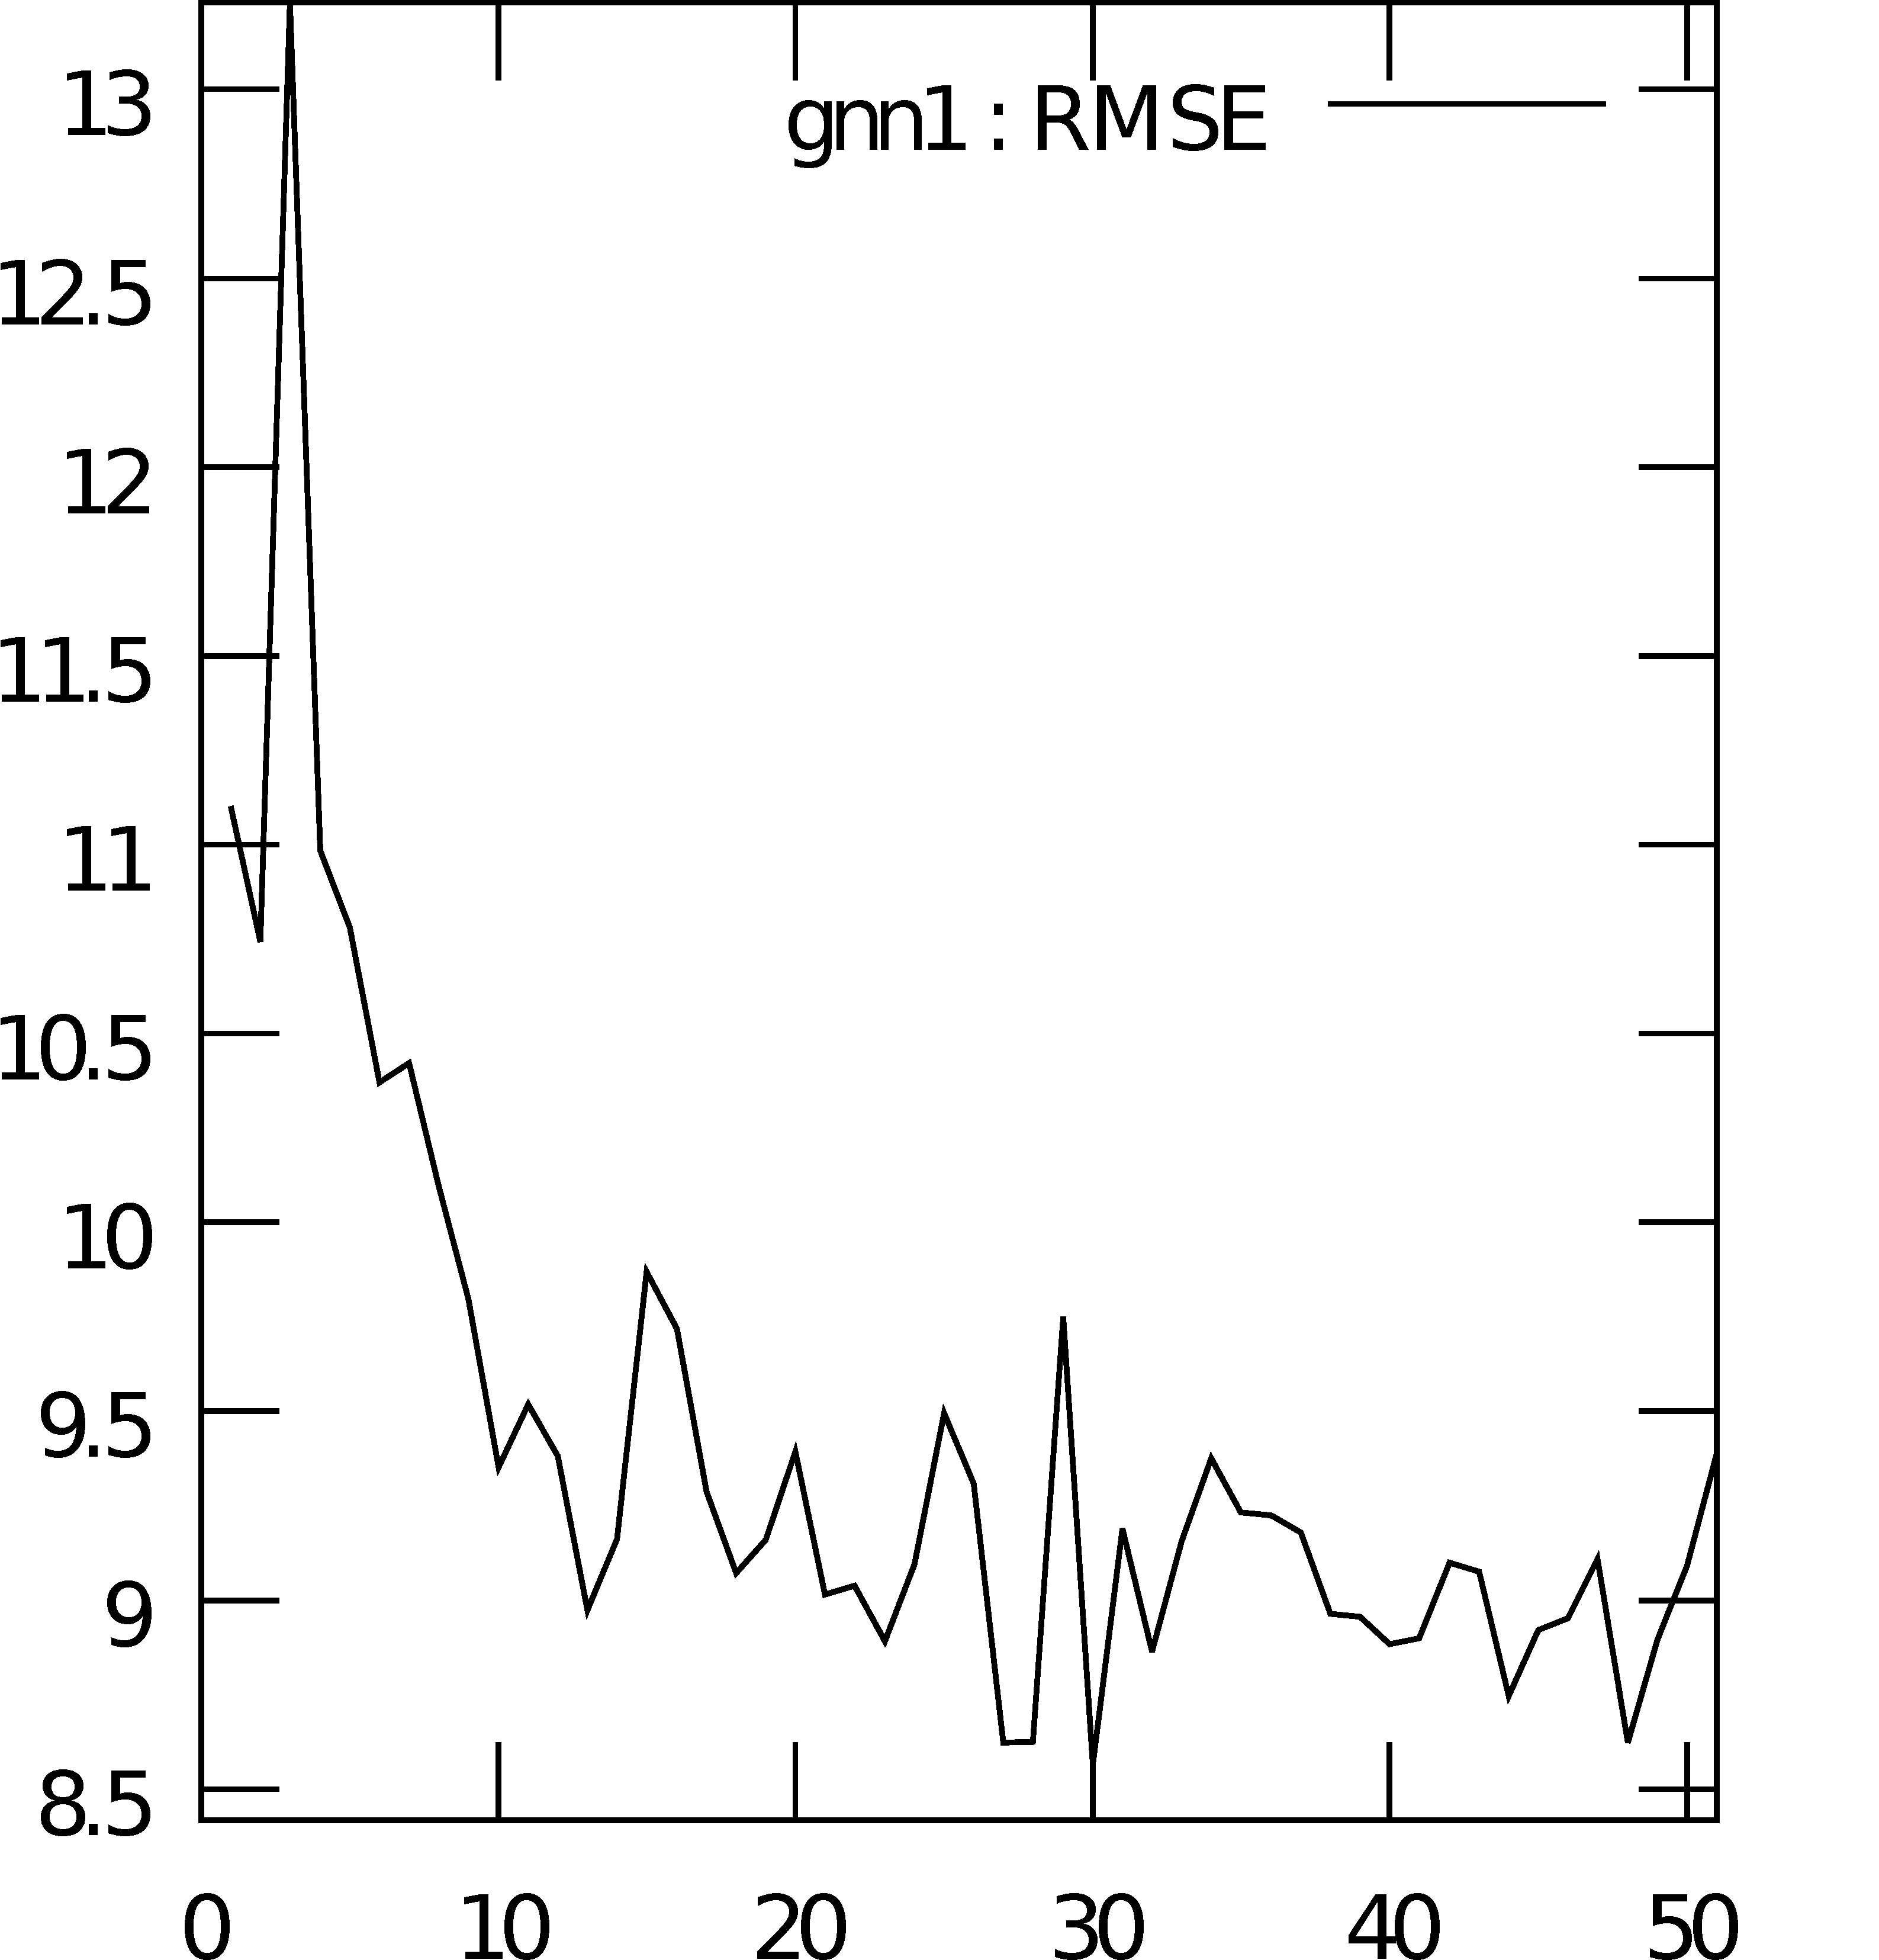
\includegraphics[scale=0.07]{img/rmse1_clipped1}
	\caption{GNN performance with $\mu = 1.2$}
	\label{fig:rmse1}
\end{center}
\end{figure}

\begin{figure}
\begin{center}
	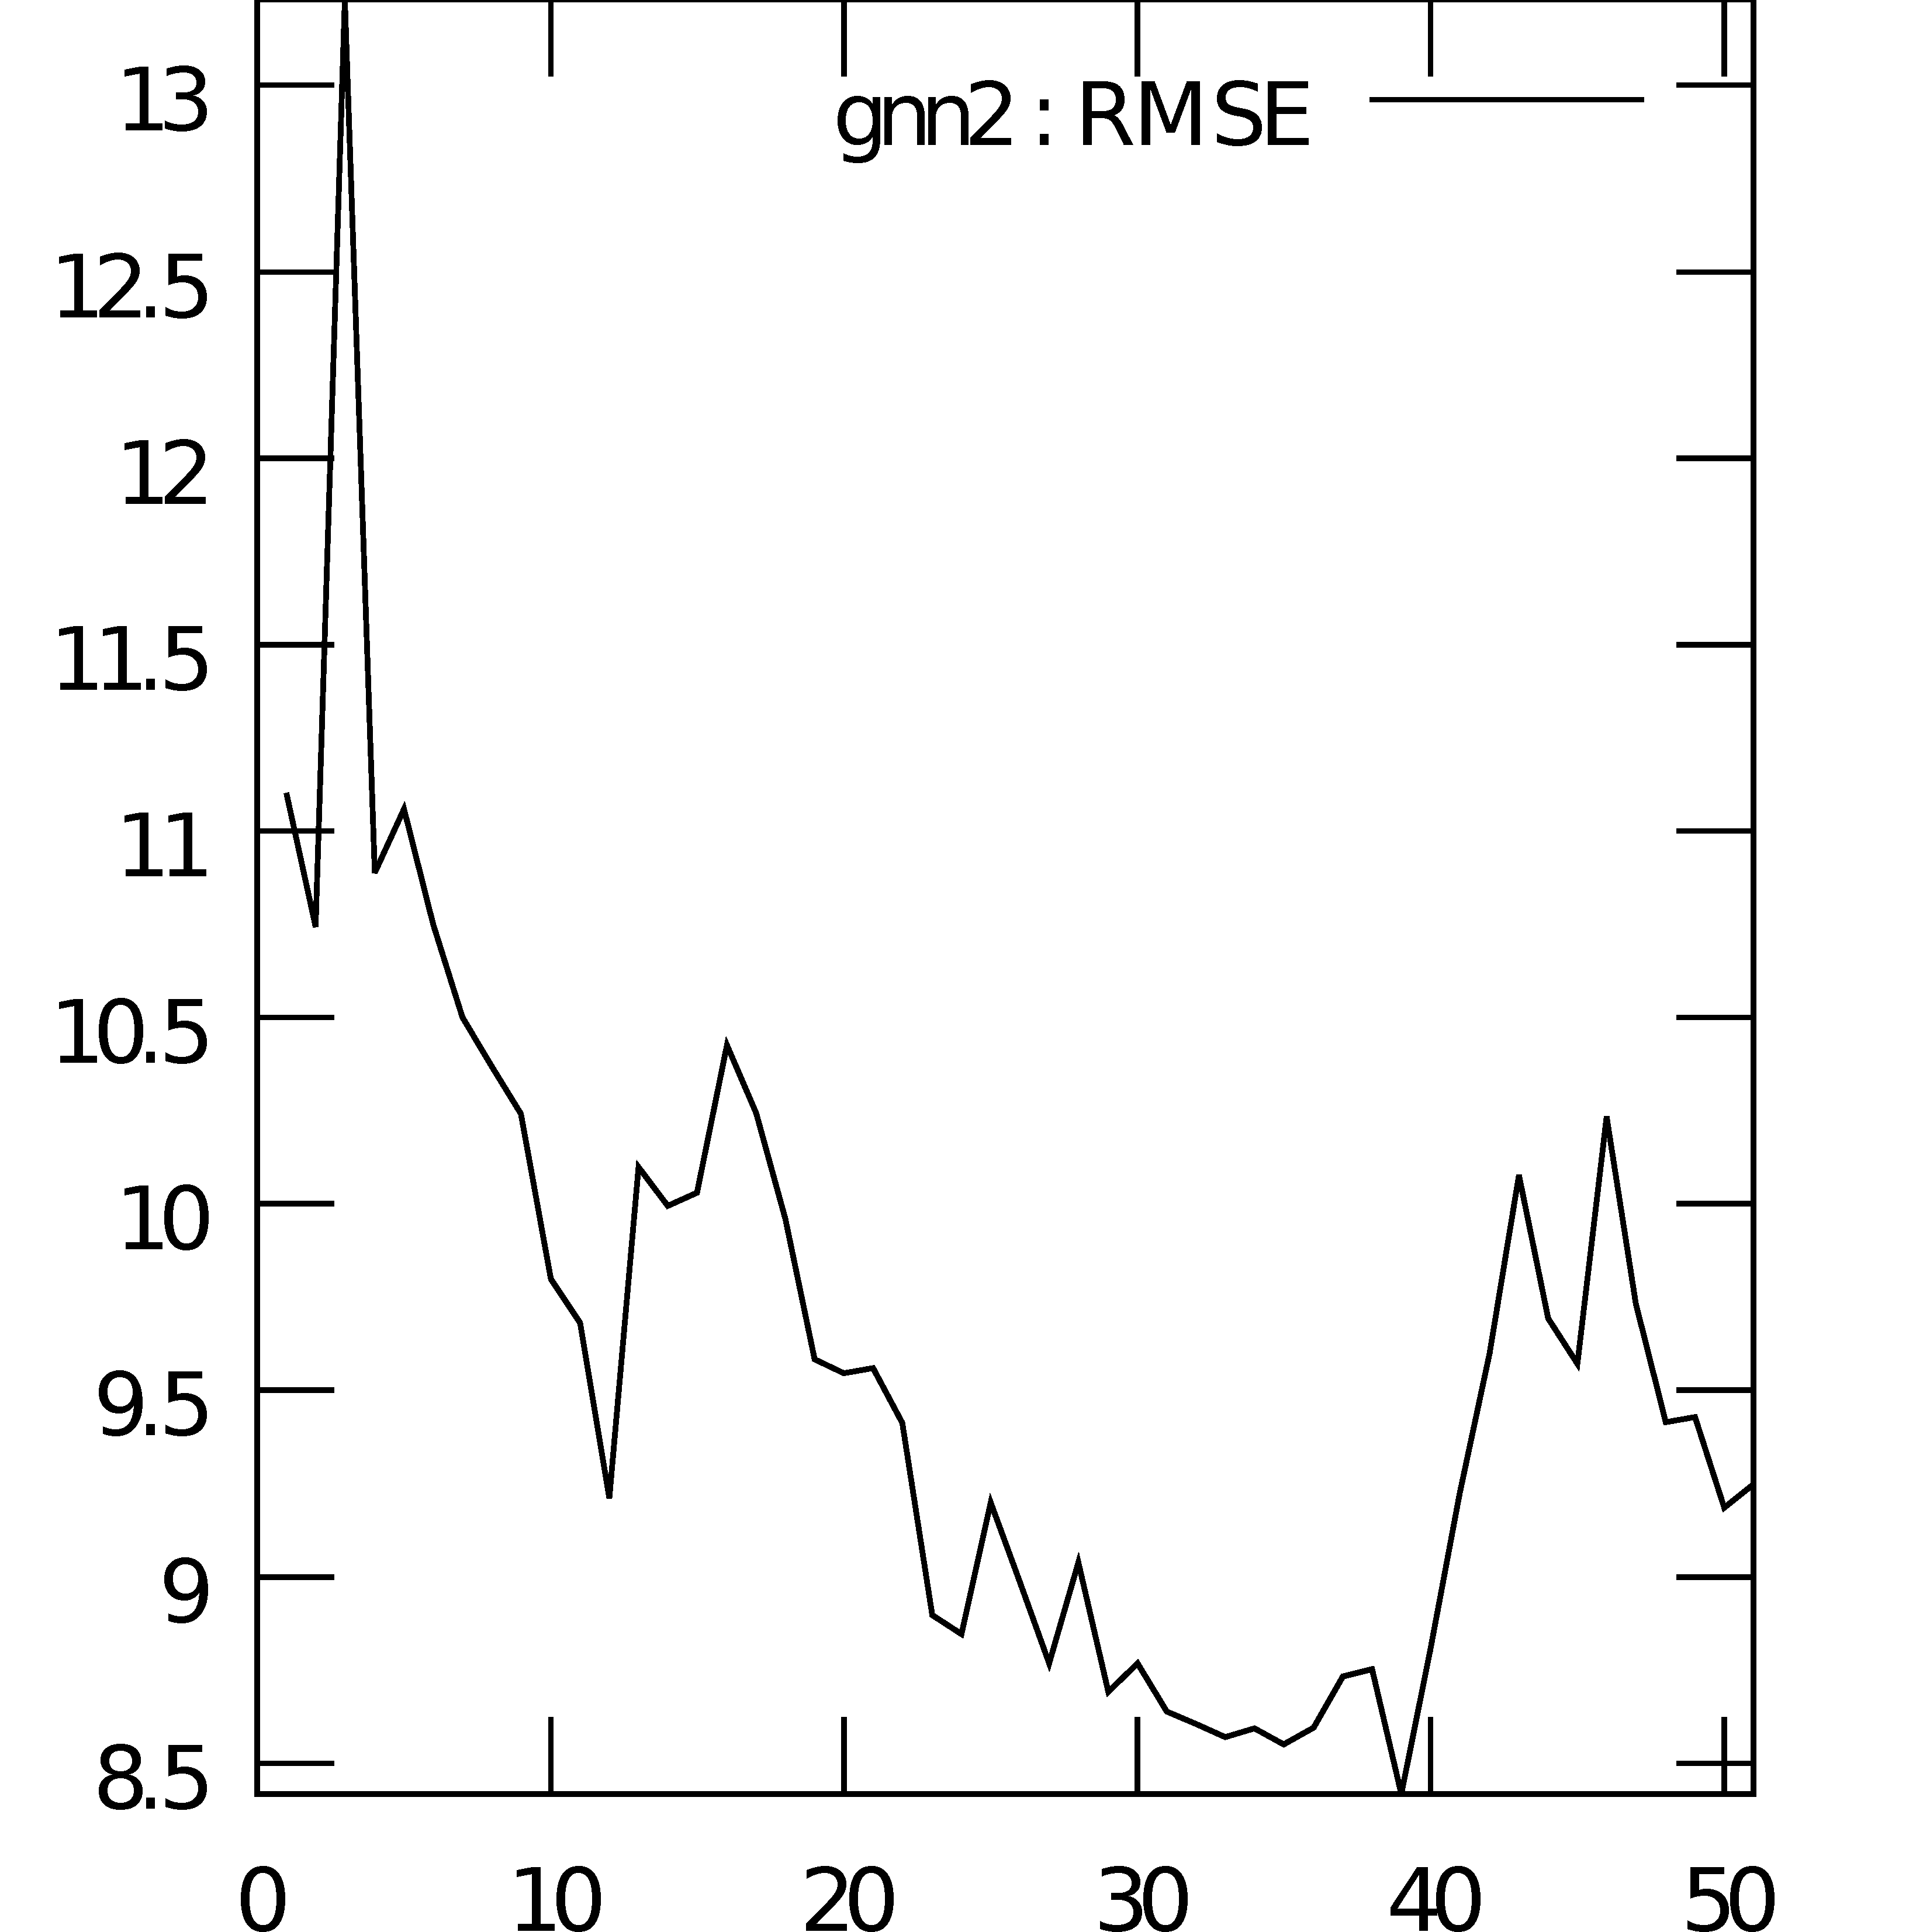
\includegraphics[scale=0.07]{img/rmse1_clipped2}
	\caption{GNN performance with $\mu = 0.9$}
	\label{fig:rmse2}
\end{center}
\end{figure}

\begin{figure}
\begin{center}
	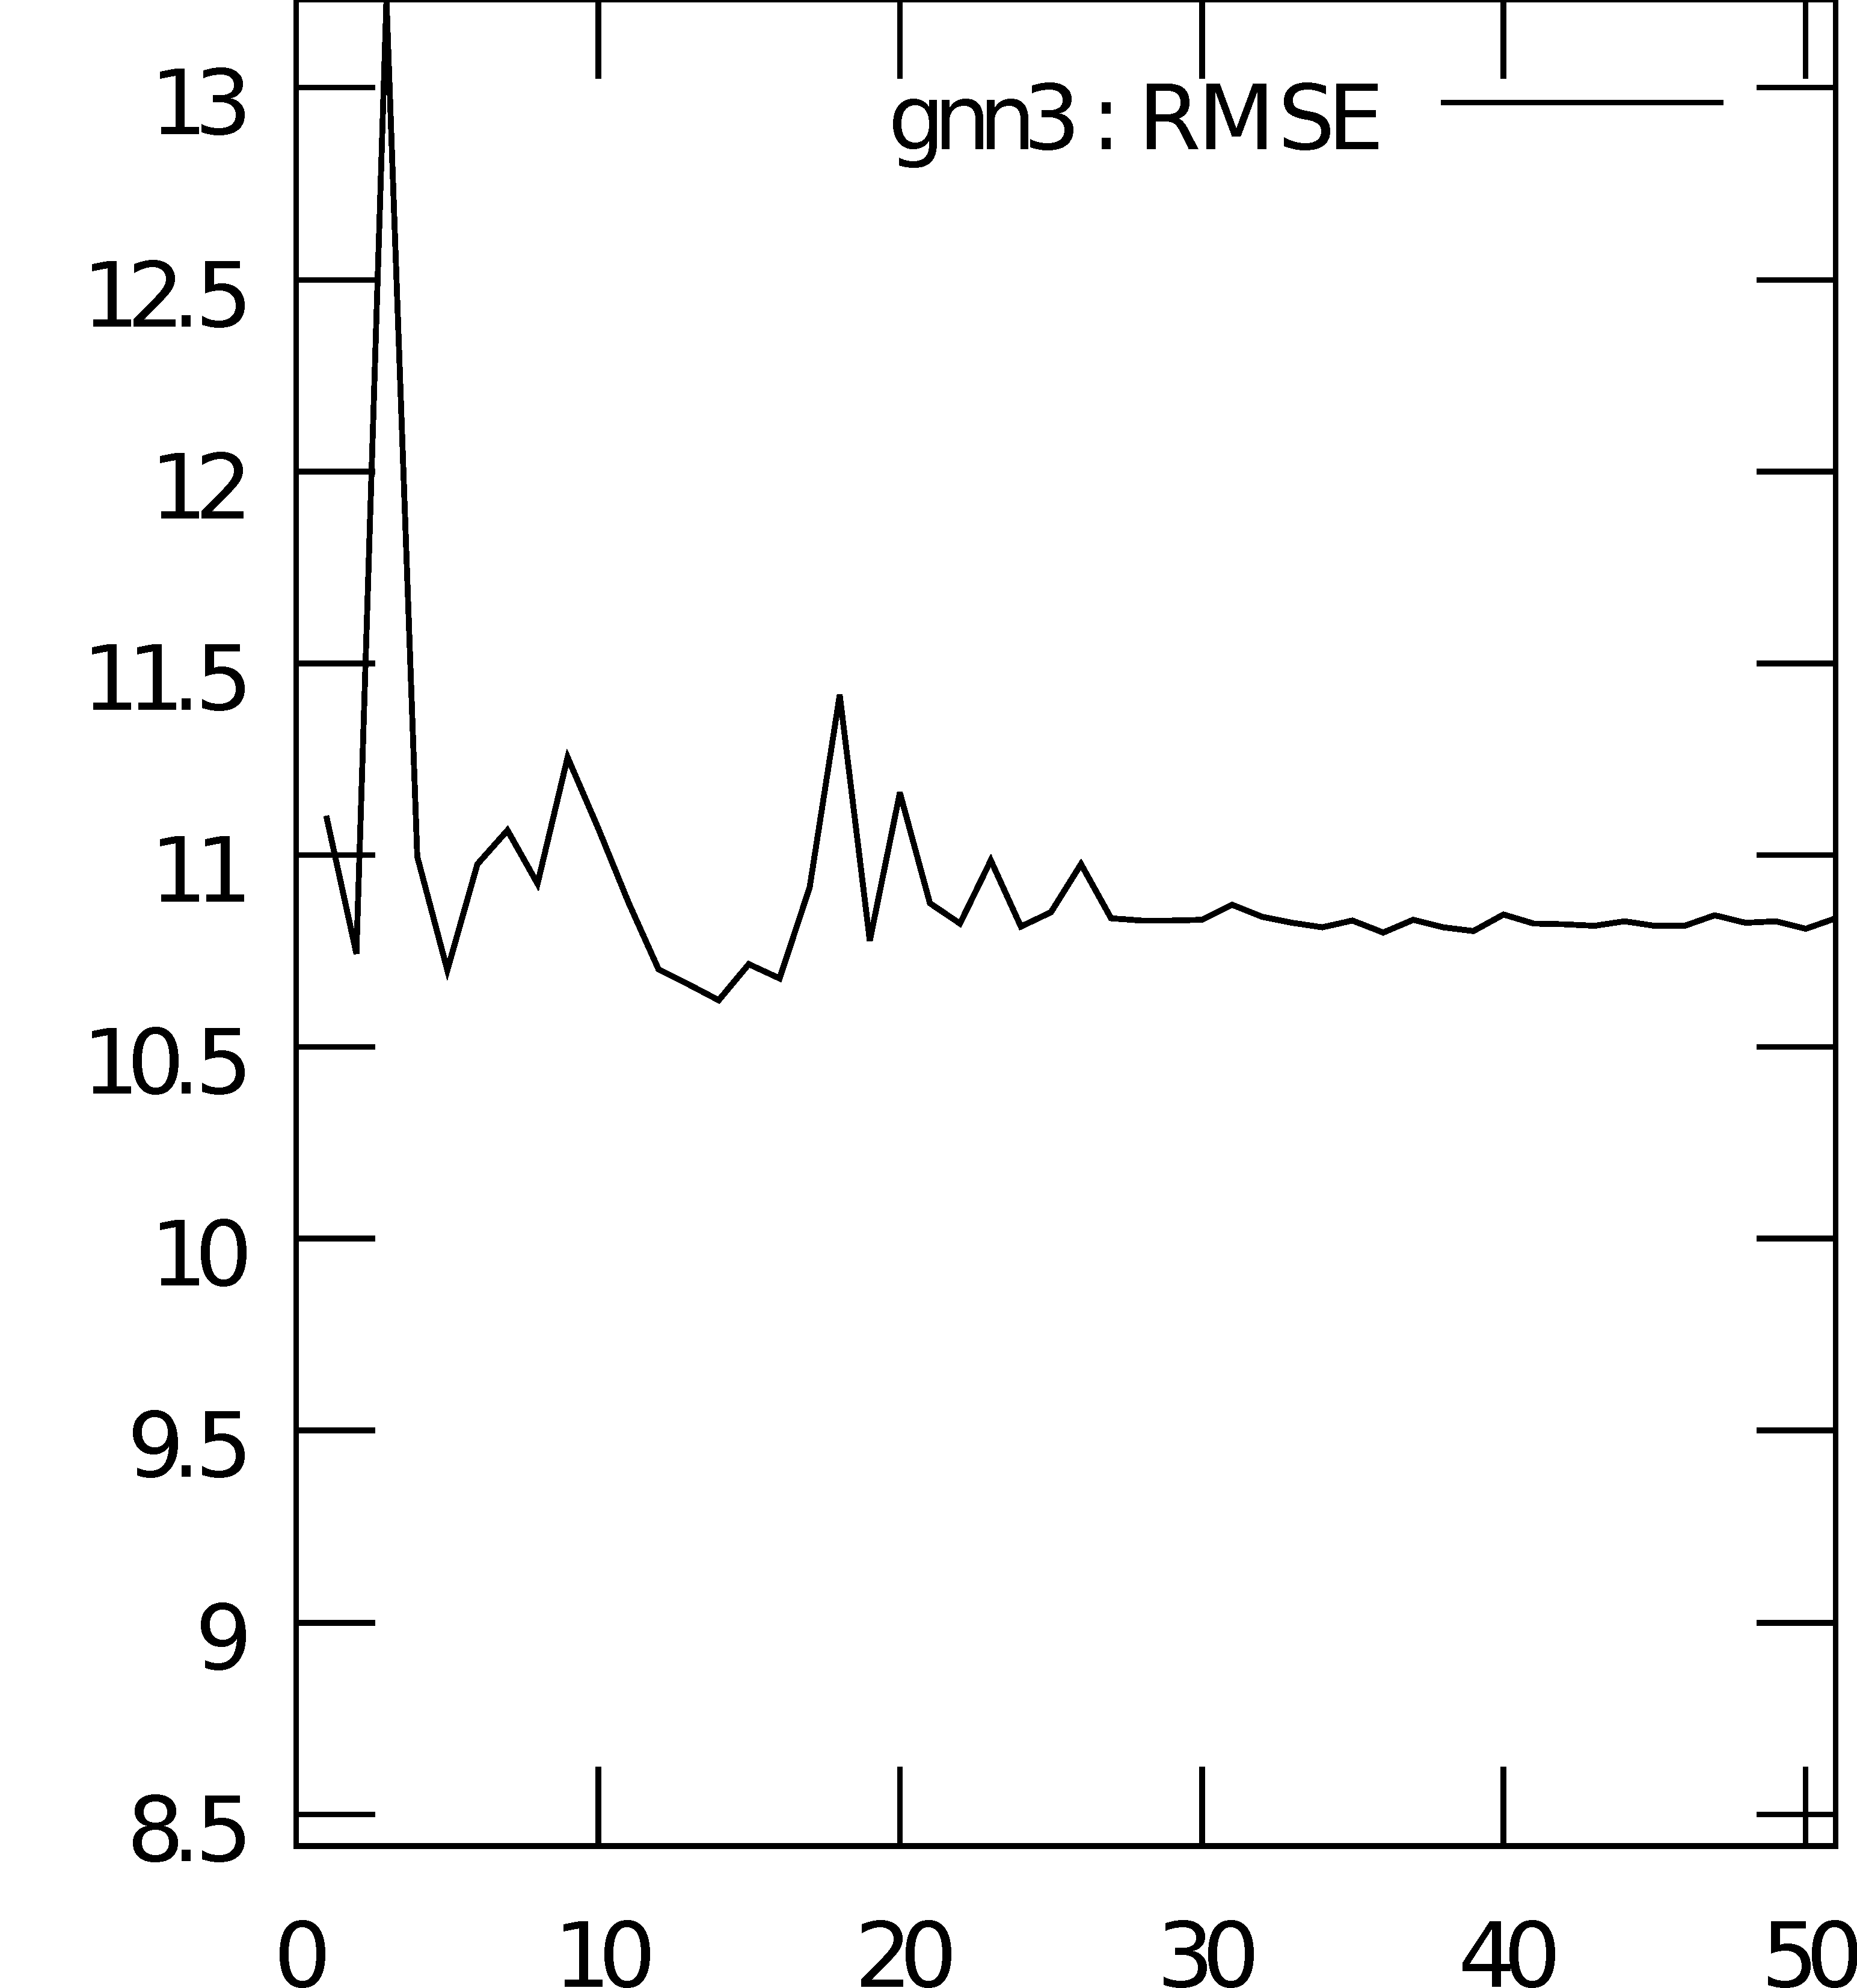
\includegraphics[scale=0.07]{img/rmse1_clipped3}
	\caption{GNN performance with $\mu = 0.6$}
	\label{fig:rmse3}
\end{center}
\end{figure}

\section{Sample results.}
To assure good classification properties, comparable with these described in the original article~\cite{scarselli2009graph}, another subgraph matching experiment was conducted. Dataset consisted of 100 random graphs, each consisting of 14 nodes (node labels [0..10] edge probability 0.2), the subgraph inserted consisted of 7 nodes. A 5-fold crossvalidation was performed on the dataset, using a random GNN with $\mu = 0.9$. For comparison, a 5-fold crossvalidation was performed on the node labels using a feedforward neural network from the Octave Neural Networks package (10 random FNNs, the one with best crossvalidation results was selected). The results are presented int Table~\ref{tab:crossmean} and Table~\ref{tab:crossstd}. The GNN performed much better than the FNN, due to taking into account graph topology. No overfitting occured. These results are comparable with the original ones.

\begin{table}[h!]
	\begin{center}
	\begin{tabular}{llll}
	\toprule
	& accuracy & precision & recall \\
	\midrule
	FNN - tr &	71\% &  65\% & 93\% \\
	FNN - tst &	71\% &  64\% &  93\% \\
	GNN - tr &	91\% &  87\%&  97\% \\
	GNN - tst &	91\% &  86\% &  97\% \\
	\bottomrule
	\end{tabular}
	\caption{Mean values on training and test sets}
	\label{tab:crossmean}
	\end{center}
\end{table}

\begin{table}[h!]
	\begin{center}
	\begin{tabular}{llll}
	\toprule
	& accuracy & precision & recall \\
	\midrule
	FNN - tr &	0.34\% &  0.67\% & 1.86\% \\
	FNN - tst &	2.45\% &  1.73\% &  2.93\% \\
	GNN - tr &	1.62\% &  1.71\% &  2.07\% \\
	GNN - tst &	3.06\% &  3.70\% &  1.39\% \\
	\bottomrule
	\end{tabular}
	\caption{Standard deviations on training and test sets}
	\label{tab:crossstd}
	\end{center}
\end{table}

\section{Conclusion.}
Implementation of a GNN requires making a couple important decisions which may affect the quality of the classifier results and the computation time. The use of a GNN for a specific dataset may require tuning the GNN parameters, especially the contraction constant $\mu$. Some observations were made concerning the behaviour of a GNN, depending on the value of its parameters:
\begin{itemize}
	\item The best training effect happens when $F_w$ remains a contraction map
	\item If $F_w$ definitely ceases to be a contraction map, there are no training effects
	\item Remaining near the contraction state can still yield good results
	\item A fixed maximum number of Forward/Backward steps can still yield good results
	\item Imposing penalty when it isn't necessary should be avoided
	\item Too large penalties (too small $\mu$) should be avoided
	\item The minimum value of $\mu$ should be tuned for the chosen dataset
	\item The minimum value of $\mu$ can be tuned on a subset of data
\end{itemize}
Some other parameters of the GNN model, such as minimum difference between states to distinguish them as different, minimum difference between error accumulator values, the influence of choosing different penalty functions, the influence of initial states are not well known and can still be investigated.


%%%%%%%%%%%%%%%%%%%%%%%%%%%%%%%%%%%%%%%%%%%%%%%%%%%%%%%%%%%%%
%%%%% References %%%%%

\bibliography{bib/gnn}
\bibliographystyle{spiebib}   %>>>> makes bibtex use spiebib.bst

\end{document} 
